% This LaTeX was auto-generated from MATLAB code.
% To make changes, update the MATLAB code and export to LaTeX again.

\documentclass{article}

\usepackage[utf8]{inputenc}
\usepackage[T1]{fontenc}
\usepackage{lmodern}
\usepackage{graphicx}
\usepackage{color}
\usepackage{hyperref}
\usepackage{amsmath}
\usepackage{amsfonts}
\usepackage{epstopdf}
\usepackage[table]{xcolor}
\usepackage{matlab}

\sloppy
\epstopdfsetup{outdir=./}
\graphicspath{ {./ass1_images/} }

\begin{document}

\begin{matlabcode}
data = csvread('2017EE10938.csv',1,1);
data
\end{matlabcode}
\begin{matlaboutput}
data = 5000x1    
   32.2681
   22.9795
   21.5283
   24.7889
   32.1239
   25.4768
   25.7775
   37.8503
   35.5771
   36.6851

\end{matlaboutput}


\vspace{1em}
\begin{matlabcode}
[D, PD] = allfitdist(data, 'PDF')
\end{matlabcode}
\begin{center}
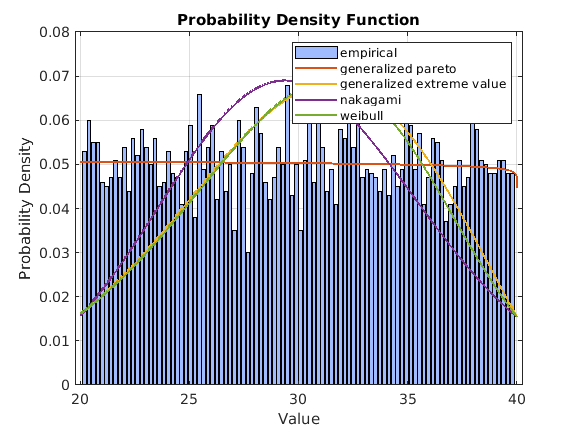
\includegraphics[width=\maxwidth{57.90265930757652em}]{figure_0.png}
\end{center}
\begin{matlabtableoutput}
{
\begin{tabular} {|c|c|c|c|c|c|c|c|c|c|c|c|}\hline
\mlcell{Fields} & \mlcell{DistName} & \mlcell{NLogL} & \mlcell{BIC} & \mlcell{AIC} & \mlcell{AICc} & \mlcell{ParamNames} & \mlcell{ParamDescription} & \mlcell{Params} & \mlcell{Paramci} & \mlcell{ParamCov} & \mlcell{Support} \\ \hline
\mlcell{1} & \mlcell{'generalized pareto'} & \mlcell{1.4976e+04} & \mlcell{2.9978e+04} & \mlcell{2.9959e+04} & \mlcell{2.9959e+04} & \mlcell{1x3 cell} & \mlcell{1x3 cell} & \mlcell{[-0.9903,19.7973,20.0067]} & \mlcell{[-1.0181,19.2491,20.0067;-0.9625,20.3611,20.0067]} & \mlcell{[0.0002,-0.0040,0;-0.0040,0.0805,0;0,0,0]} & \mlcell{1x1 struct} \\ \hline
\mlcell{2} & \mlcell{'generalized extreme value'} & \mlcell{1.5725e+04} & \mlcell{3.1476e+04} & \mlcell{3.1456e+04} & \mlcell{3.1456e+04} & \mlcell{1x3 cell} & \mlcell{1x3 cell} & \mlcell{[-0.4403,6.0702,28.3747]} & \mlcell{[-0.4711,5.9091,28.1771;-0.4096,6.2357,28.5723]} & \mlcell{[2.4612e-04,-0.0010,-0.0008;-9.7560e-04,0.0069,0.0004;-8.1014e-04,0.0004,0.0102]} & \mlcell{1x1 struct} \\ \hline
\mlcell{3} & \mlcell{'nakagami'} & \mlcell{1.5842e+04} & \mlcell{3.1702e+04} & \mlcell{3.1689e+04} & \mlcell{3.1689e+04} & \mlcell{1x2 cell} & \mlcell{1x2 cell} & \mlcell{[6.8530,930.9644]} & \mlcell{[6.5956,921.1591;7.1204,940.8740]} & \mlcell{[0.0179,0.0000;0.0000,25.2941]} & \mlcell{1x1 struct} \\ \hline
\mlcell{4} & \mlcell{'weibull'} & \mlcell{1.5845e+04} & \mlcell{3.1708e+04} & \mlcell{3.1695e+04} & \mlcell{3.1695e+04} & \mlcell{1x2 cell} & \mlcell{1x2 cell} & \mlcell{[32.3537,5.9416]} & \mlcell{[32.1946,5.8125;32.5135,6.0736]} & \mlcell{[0.0066,0.0017;0.0017,0.0044]} & \mlcell{1x1 struct} \\ \hline
\mlcell{5} & \mlcell{'rician'} & \mlcell{1.5853e+04} & \mlcell{3.1724e+04} & \mlcell{3.1711e+04} & \mlcell{3.1711e+04} & \mlcell{1x2 cell} & \mlcell{1x2 cell} & \mlcell{[29.3782,5.8260]} & \mlcell{[29.2133,5.7105;29.5431,5.9439]} & \mlcell{[0.0071,-0.0007;-0.0007,0.0035]} & \mlcell{1x1 struct} \\ \hline
\mlcell{6} & \mlcell{'normal'} & \mlcell{1.5855e+04} & \mlcell{3.1726e+04} & \mlcell{3.1713e+04} & \mlcell{3.1713e+04} & \mlcell{1x2 cell} & \mlcell{1x2 cell} & \mlcell{[29.9619,5.7666]} & \mlcell{[29.8021,5.6557;30.1218,5.8819]} & \mlcell{[0.0067,-0.0000;-0.0000,0.0033]} & \mlcell{1x1 struct} \\ \hline
\mlcell{7} & \mlcell{'tlocationscale'} & \mlcell{1.5855e+04} & \mlcell{3.1735e+04} & \mlcell{3.1715e+04} & \mlcell{3.1715e+04} & \mlcell{1x3 cell} & \mlcell{1x3 cell} & \mlcell{[29.9623,5.7661,4.2957e+06]} & \mlcell{[-Inf,-Inf,-Inf;Inf,Inf,Inf]} & \mlcell{[NaN,NaN,NaN;NaN,NaN,NaN;NaN,NaN,NaN]} & \mlcell{1x1 struct} \\ \hline
\mlcell{8} & \mlcell{'gamma'} & \mlcell{1.5863e+04} & \mlcell{3.1743e+04} & \mlcell{3.1730e+04} & \mlcell{3.1730e+04} & \mlcell{1x2 cell} & \mlcell{1x2 cell} & \mlcell{[26.2298,1.1423]} & \mlcell{[25.2277,1.0982;27.2716,1.1881]} & \mlcell{[0.2717,-0.0118;-0.0118,0.0005]} & \mlcell{1x1 struct} \\ \hline
\mlcell{9} & \mlcell{'birnbaumsaunders'} & \mlcell{1.5888e+04} & \mlcell{3.1792e+04} & \mlcell{3.1779e+04} & \mlcell{3.1779e+04} & \mlcell{1x2 cell} & \mlcell{1x2 cell} & \mlcell{[29.3833,0.1984]} & \mlcell{[29.2225,0.1945;29.5441,0.2023]} & \mlcell{[0.0067,-5.3528e-09;-0.0000,3.9376e-06]} & \mlcell{1x1 struct} \\ \hline
\mlcell{10} & \mlcell{'inverse gaussian'} & \mlcell{1.5888e+04} & \mlcell{3.1794e+04} & \mlcell{3.1781e+04} & \mlcell{3.1781e+04} & \mlcell{1x2 cell} & \mlcell{1x2 cell} & \mlcell{[29.9619,753.5083]} & \mlcell{[29.7963,723.9713;30.1275,783.0452]} & \mlcell{[0.0071,0.0000;0.0000,227.1098]} & \mlcell{1x1 struct} \\ \hline
\mlcell{11} & \mlcell{'lognormal'} & \mlcell{1.5897e+04} & \mlcell{3.1810e+04} & \mlcell{3.1797e+04} & \mlcell{3.1797e+04} & \mlcell{1x2 cell} & \mlcell{1x2 cell} & \mlcell{[3.3807,0.1978]} & \mlcell{[3.3753,0.1940;3.3862,0.2018]} & \mlcell{[7.8285e-06,-2.9112e-20;-2.9112e-20,3.9154e-06]} & \mlcell{1x1 struct} \\ \hline
\mlcell{12} & \mlcell{'extreme value'} & \mlcell{1.6006e+04} & \mlcell{3.2029e+04} & \mlcell{3.2016e+04} & \mlcell{3.2016e+04} & \mlcell{1x2 cell} & \mlcell{1x2 cell} & \mlcell{[32.8298,5.2117]} & \mlcell{[32.6769,5.1010;32.9828,5.3248]} & \mlcell{[0.0061,-0.0015;-0.0015,0.0033]} & \mlcell{1x1 struct} \\ \hline
\mlcell{13} & \mlcell{'logistic'} & \mlcell{1.6080e+04} & \mlcell{3.2176e+04} & \mlcell{3.2163e+04} & \mlcell{3.2163e+04} & \mlcell{1x2 cell} & \mlcell{1x2 cell} & \mlcell{[29.9685,3.5038]} & \mlcell{[29.7948,3.4263;30.1422,3.5830]} & \mlcell{[0.0079,-0.0000;-0.0000,0.0016]} & \mlcell{1x1 struct} \\ \hline
\mlcell{14} & \mlcell{'loglogistic'} & \mlcell{1.6107e+04} & \mlcell{3.2231e+04} & \mlcell{3.2218e+04} & \mlcell{3.2218e+04} & \mlcell{1x2 cell} & \mlcell{1x2 cell} & \mlcell{[3.3881,0.1195]} & \mlcell{[3.3822,0.1169;3.3940,0.1223]} & \mlcell{[9.1119e-06,-1.5281e-07;-1.5281e-07,1.8718e-06]} & \mlcell{1x1 struct} \\ 
\hline
\end{tabular}
}
{
\begin{tabular} {|c|c|c|c|c|c|c|c|c|c|c|c|c|c|c|c|c|}\hline
\mlcell{ } & \mlcell{1} & \mlcell{2} & \mlcell{3} & \mlcell{4} & \mlcell{5} & \mlcell{6} & \mlcell{7} & \mlcell{8} & \mlcell{9} & \mlcell{10} & \mlcell{11} & \mlcell{12} & \mlcell{13} & \mlcell{14} & \mlcell{15} & \mlcell{16} \\ \hline
\mlcell{1} & \mlcell{1x1 GeneralizedParetoDistribution} & \mlcell{1x1 GeneralizedExtremeValueDistribution} & \mlcell{1x1 NakagamiDistribution} & \mlcell{1x1 WeibullDistribution} & \mlcell{1x1 RicianDistribution} & \mlcell{1x1 NormalDistribution} & \mlcell{1x1 tLocationScaleDistribution} & \mlcell{1x1 GammaDistribution} & \mlcell{1x1 BirnbaumSaundersDistribution} & \mlcell{1x1 InverseGaussianDistribution} & \mlcell{1x1 LognormalDistribution} & \mlcell{1x1 ExtremeValueDistribution} & \mlcell{1x1 LogisticDistribution} & \mlcell{1x1 LoglogisticDistribution} & \mlcell{1x1 RayleighDistribution} & \mlcell{1x1 ExponentialDistribution} \\ 
\hline
\end{tabular}
}
\end{matlabtableoutput}
\begin{matlabcode}
[D, PD] = allfitdist(data, 'CDF')
\end{matlabcode}
\begin{center}
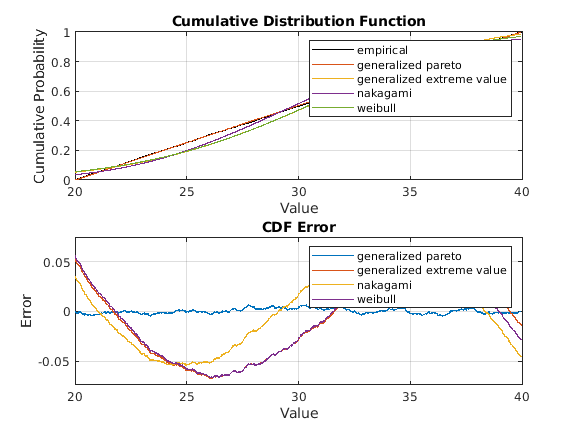
\includegraphics[width=\maxwidth{57.90265930757652em}]{figure_1.png}
\end{center}
\begin{matlabtableoutput}
{
\begin{tabular} {|c|c|c|c|c|c|c|c|c|c|c|c|}\hline
\mlcell{Fields} & \mlcell{DistName} & \mlcell{NLogL} & \mlcell{BIC} & \mlcell{AIC} & \mlcell{AICc} & \mlcell{ParamNames} & \mlcell{ParamDescription} & \mlcell{Params} & \mlcell{Paramci} & \mlcell{ParamCov} & \mlcell{Support} \\ \hline
\mlcell{1} & \mlcell{'generalized pareto'} & \mlcell{1.4976e+04} & \mlcell{2.9978e+04} & \mlcell{2.9959e+04} & \mlcell{2.9959e+04} & \mlcell{1x3 cell} & \mlcell{1x3 cell} & \mlcell{[-0.9903,19.7973,20.0067]} & \mlcell{[-1.0181,19.2491,20.0067;-0.9625,20.3611,20.0067]} & \mlcell{[0.0002,-0.0040,0;-0.0040,0.0805,0;0,0,0]} & \mlcell{1x1 struct} \\ \hline
\mlcell{2} & \mlcell{'generalized extreme value'} & \mlcell{1.5725e+04} & \mlcell{3.1476e+04} & \mlcell{3.1456e+04} & \mlcell{3.1456e+04} & \mlcell{1x3 cell} & \mlcell{1x3 cell} & \mlcell{[-0.4403,6.0702,28.3747]} & \mlcell{[-0.4711,5.9091,28.1771;-0.4096,6.2357,28.5723]} & \mlcell{[2.4612e-04,-0.0010,-0.0008;-9.7560e-04,0.0069,0.0004;-8.1014e-04,0.0004,0.0102]} & \mlcell{1x1 struct} \\ \hline
\mlcell{3} & \mlcell{'nakagami'} & \mlcell{1.5842e+04} & \mlcell{3.1702e+04} & \mlcell{3.1689e+04} & \mlcell{3.1689e+04} & \mlcell{1x2 cell} & \mlcell{1x2 cell} & \mlcell{[6.8530,930.9644]} & \mlcell{[6.5956,921.1591;7.1204,940.8740]} & \mlcell{[0.0179,0.0000;0.0000,25.2941]} & \mlcell{1x1 struct} \\ \hline
\mlcell{4} & \mlcell{'weibull'} & \mlcell{1.5845e+04} & \mlcell{3.1708e+04} & \mlcell{3.1695e+04} & \mlcell{3.1695e+04} & \mlcell{1x2 cell} & \mlcell{1x2 cell} & \mlcell{[32.3537,5.9416]} & \mlcell{[32.1946,5.8125;32.5135,6.0736]} & \mlcell{[0.0066,0.0017;0.0017,0.0044]} & \mlcell{1x1 struct} \\ \hline
\mlcell{5} & \mlcell{'rician'} & \mlcell{1.5853e+04} & \mlcell{3.1724e+04} & \mlcell{3.1711e+04} & \mlcell{3.1711e+04} & \mlcell{1x2 cell} & \mlcell{1x2 cell} & \mlcell{[29.3782,5.8260]} & \mlcell{[29.2133,5.7105;29.5431,5.9439]} & \mlcell{[0.0071,-0.0007;-0.0007,0.0035]} & \mlcell{1x1 struct} \\ \hline
\mlcell{6} & \mlcell{'normal'} & \mlcell{1.5855e+04} & \mlcell{3.1726e+04} & \mlcell{3.1713e+04} & \mlcell{3.1713e+04} & \mlcell{1x2 cell} & \mlcell{1x2 cell} & \mlcell{[29.9619,5.7666]} & \mlcell{[29.8021,5.6557;30.1218,5.8819]} & \mlcell{[0.0067,-0.0000;-0.0000,0.0033]} & \mlcell{1x1 struct} \\ \hline
\mlcell{7} & \mlcell{'tlocationscale'} & \mlcell{1.5855e+04} & \mlcell{3.1735e+04} & \mlcell{3.1715e+04} & \mlcell{3.1715e+04} & \mlcell{1x3 cell} & \mlcell{1x3 cell} & \mlcell{[29.9623,5.7661,4.2957e+06]} & \mlcell{[-Inf,-Inf,-Inf;Inf,Inf,Inf]} & \mlcell{[NaN,NaN,NaN;NaN,NaN,NaN;NaN,NaN,NaN]} & \mlcell{1x1 struct} \\ \hline
\mlcell{8} & \mlcell{'gamma'} & \mlcell{1.5863e+04} & \mlcell{3.1743e+04} & \mlcell{3.1730e+04} & \mlcell{3.1730e+04} & \mlcell{1x2 cell} & \mlcell{1x2 cell} & \mlcell{[26.2298,1.1423]} & \mlcell{[25.2277,1.0982;27.2716,1.1881]} & \mlcell{[0.2717,-0.0118;-0.0118,0.0005]} & \mlcell{1x1 struct} \\ \hline
\mlcell{9} & \mlcell{'birnbaumsaunders'} & \mlcell{1.5888e+04} & \mlcell{3.1792e+04} & \mlcell{3.1779e+04} & \mlcell{3.1779e+04} & \mlcell{1x2 cell} & \mlcell{1x2 cell} & \mlcell{[29.3833,0.1984]} & \mlcell{[29.2225,0.1945;29.5441,0.2023]} & \mlcell{[0.0067,-5.3528e-09;-0.0000,3.9376e-06]} & \mlcell{1x1 struct} \\ \hline
\mlcell{10} & \mlcell{'inverse gaussian'} & \mlcell{1.5888e+04} & \mlcell{3.1794e+04} & \mlcell{3.1781e+04} & \mlcell{3.1781e+04} & \mlcell{1x2 cell} & \mlcell{1x2 cell} & \mlcell{[29.9619,753.5083]} & \mlcell{[29.7963,723.9713;30.1275,783.0452]} & \mlcell{[0.0071,0.0000;0.0000,227.1098]} & \mlcell{1x1 struct} \\ \hline
\mlcell{11} & \mlcell{'lognormal'} & \mlcell{1.5897e+04} & \mlcell{3.1810e+04} & \mlcell{3.1797e+04} & \mlcell{3.1797e+04} & \mlcell{1x2 cell} & \mlcell{1x2 cell} & \mlcell{[3.3807,0.1978]} & \mlcell{[3.3753,0.1940;3.3862,0.2018]} & \mlcell{[7.8285e-06,-2.9112e-20;-2.9112e-20,3.9154e-06]} & \mlcell{1x1 struct} \\ \hline
\mlcell{12} & \mlcell{'extreme value'} & \mlcell{1.6006e+04} & \mlcell{3.2029e+04} & \mlcell{3.2016e+04} & \mlcell{3.2016e+04} & \mlcell{1x2 cell} & \mlcell{1x2 cell} & \mlcell{[32.8298,5.2117]} & \mlcell{[32.6769,5.1010;32.9828,5.3248]} & \mlcell{[0.0061,-0.0015;-0.0015,0.0033]} & \mlcell{1x1 struct} \\ \hline
\mlcell{13} & \mlcell{'logistic'} & \mlcell{1.6080e+04} & \mlcell{3.2176e+04} & \mlcell{3.2163e+04} & \mlcell{3.2163e+04} & \mlcell{1x2 cell} & \mlcell{1x2 cell} & \mlcell{[29.9685,3.5038]} & \mlcell{[29.7948,3.4263;30.1422,3.5830]} & \mlcell{[0.0079,-0.0000;-0.0000,0.0016]} & \mlcell{1x1 struct} \\ \hline
\mlcell{14} & \mlcell{'loglogistic'} & \mlcell{1.6107e+04} & \mlcell{3.2231e+04} & \mlcell{3.2218e+04} & \mlcell{3.2218e+04} & \mlcell{1x2 cell} & \mlcell{1x2 cell} & \mlcell{[3.3881,0.1195]} & \mlcell{[3.3822,0.1169;3.3940,0.1223]} & \mlcell{[9.1119e-06,-1.5281e-07;-1.5281e-07,1.8718e-06]} & \mlcell{1x1 struct} \\ 
\hline
\end{tabular}
}
{
\begin{tabular} {|c|c|c|c|c|c|c|c|c|c|c|c|c|c|c|c|c|}\hline
\mlcell{ } & \mlcell{1} & \mlcell{2} & \mlcell{3} & \mlcell{4} & \mlcell{5} & \mlcell{6} & \mlcell{7} & \mlcell{8} & \mlcell{9} & \mlcell{10} & \mlcell{11} & \mlcell{12} & \mlcell{13} & \mlcell{14} & \mlcell{15} & \mlcell{16} \\ \hline
\mlcell{1} & \mlcell{1x1 GeneralizedParetoDistribution} & \mlcell{1x1 GeneralizedExtremeValueDistribution} & \mlcell{1x1 NakagamiDistribution} & \mlcell{1x1 WeibullDistribution} & \mlcell{1x1 RicianDistribution} & \mlcell{1x1 NormalDistribution} & \mlcell{1x1 tLocationScaleDistribution} & \mlcell{1x1 GammaDistribution} & \mlcell{1x1 BirnbaumSaundersDistribution} & \mlcell{1x1 InverseGaussianDistribution} & \mlcell{1x1 LognormalDistribution} & \mlcell{1x1 ExtremeValueDistribution} & \mlcell{1x1 LogisticDistribution} & \mlcell{1x1 LoglogisticDistribution} & \mlcell{1x1 RayleighDistribution} & \mlcell{1x1 ExponentialDistribution} \\ 
\hline
\end{tabular}
}
\end{matlabtableoutput}

\end{document}
